\documentclass[11pt]{article}

%\usepackage[utf8]{inputenc}
\usepackage{deauthor}
\usepackage{authblk}
\usepackage{times,graphicx}
\usepackage{multirow}
\usepackage{amssymb} %checkmark
\usepackage{xspace}

\graphicspath{{submissions/eda-survey-peng}}

\newcommand{\stitle}[1]{ \noindent{\bf #1.\xspace}}

\begin{document}

\title{User Interfaces for Exploratory Data Analysis: A Survey of \\ Open-Source and Commercial Tools}

\author{Jinglin Peng$^{\dagger}$\thanks{ The first two authors contributed equally to this work.} 
\hspace{2em} Weiyuan Wu$^{\dagger*}$ 
\hspace{2em} Jing Nathan Yan$^{\ddagger}$ 
\hspace{1em} Danrui Qi$^{\dagger}$ 
\hspace{1em} \\
%\vspace{-1ex}
Jeffrey M. Rzeszotarski$^{\ddagger}$ \hspace{1em} Jiannan Wang$^{\dagger}$\\
%\vspace{2ex}
$^{\dagger}$ Simon Fraser University, Canada \hspace{1em} \texttt{\small\{jinglin\_peng, youngw, dqi, jnwang\}@sfu.ca}\\
$^{\ddagger}$ Cornell University, USA \hspace{1em} \texttt{\small\{jy858, jeffrz\}@cornell.edu}
}

\maketitle



\begin{abstract}
    Exploratory Data Analysis (EDA) is an important step in data processing pipelines, for which many tools have been developed. In this article we take an initial step in evaluating the relationship between users and EDA tools, as mediated by their interfaces, across different stages of the EDA process. We compare 11 commercial and open-sourced tools, categorizing their interfaces with respect to three stages of EDA: 1) generating initial questions, 2) creating visualizations, and 3) examining visualizations. Finally, we discuss trade-offs between different interfaces, and identify future work and research opportunities for the broader EDA technical community. 
\end{abstract}


\section{Introduction}

Data processing is the procedure to transform collected raw data into useful information. When processing data in the course of conducting a broader investigation, analysts develop a pipeline or set of activities with linked outputs and inputs, for their work. 
%As shown in Figure~\ref{fig:data-pipeline}, 
A typical data processing pipeline includes acquiring data from different sources, wrangling and transforming data into a format ready for exploration, exploring data to examine its quality, discovering insights, building a model for prediction, and finally reporting results~\cite{DBLP:journals/corr/abs-1911-00568}. 


Exploratory data analysis (EDA) is an important step in the data processing pipeline, providing necessary data profiling and insight discovery prior to in-depth analysis~\cite{DBLP:journals/corr/abs-1911-00568}. A number of tools have been proposed from both academia and industry to better support end users making sense of data~\cite{powerbi, tableau, DBLP:journals/tvcg/StolteTH02, DBLP:conf/icde/LuoQ0018, DBLP:journals/pvldb/VartakRMPP15, DBLP:journals/ivs/CuiBYE19, DBLP:journals/pvldb/LeeTABCKMSYHP21, DBLP:conf/sigmod/PengWLBYXCRW21, DBLP:journals/pvldb/Kraska18, DBLP:journals/pvldb/SiddiquiKLKP16, DBLP:conf/chi/WongsuphasawatQ17, DBLP:conf/cidr/WuPMZR17, DBLP:journals/jossw/VanderPlasGHMWS18}. Prior work in this space has summarized the features of such tools based on their task affordances (e.g., univariate analysis, bivariate analysis, multivariate analysis). Researchers have also adopted a number of lenses for surveying tools. For example, Staniak et al. reviewed existing libraries by tasks that they can support~\cite{DBLP:journals/rjour/StaniakB19}, and Ghosh et al. reviewed whether existing pillars can handle the high volume of data through empirically studying 43 academic and 7 commercial tools~\cite{DBLP:journals/vi/GhoshNMQM18}. Existing work focused on the tasks into which tools can fit, however, risks overlooking or under-emphasizing the human-in-the-loop nature of EDA. The human interface of the tool is indeed the essential connection point between the system and an analyst's data processing pipeline, and merits additional investigation. In this paper, we aim through synthesizing existing pillars of tools, to understand how users make sense of data through different interfaces. As interfaces are closely tied to different EDA stages~\cite{DBLP:journals/cgf/BattleH19}, we contextualize the impact of interfaces from tools in different EDA stages of the data processing pipeline.


One key challenge we face in this work is in aligning the use of tools with stages of the EDA process. Research communities have extensively examined the EDA process, which is highly iterative and interactive, but there is no one dominant framework for the EDA process~\cite{yan2021tessera, DBLP:journals/cgf/BattleH19}. Rather, our understanding is constantly evolving in concert with tools. Early on, Tukey~\cite{martinez2017exploratory} gives one of the earliest definitions of EDA as the following process: \emph{``1) start with some ideas, 2) iterate between asking a question and creating a design, 3) collect data according to the designed experiment, 4) perform a statistical analysis of data, and 5) produce an answer"};  however, as EDA tasks and the datasets to be explored are becoming more sophisticated, recent research identifies that there might not exist schemata for the stages of EDA which are both universal and specific. For example, Shneiderman uses from the visual information seeking mantra: \emph{``overview first, zoom and filter, then details-on-demand"}~\cite{DBLP:conf/vl/Shneiderman96} instead of characterizing exact and implicit stages, and Heer et al. summarize the visual analysis process as \emph{``an iterative
process of view creation, exploration,
and refinement"}~\cite{DBLP:journals/cacm/HeerS12}.

In an effort to retain specificity in our survey while also acknowledging the reality that there is no one perfect categorization scheme for EDA, we focus on specific user exploration activities as they relate to the interfaces. In this work, we opt to adapt common definitions from Tukey and adapt them for the modern EDA context. More specifically, we remove the ``collect data" step as we consider the scenario of conducting EDA on collected data. Besides, since the recent advancement of surveyed tools are mainly about visualizations, we focus on visualizations in this work. We change ``create a design" to ``create visualizations", and combine the last two steps as ``examine visualizations". Note that there are also other ways to gain insights during EDA, such as executing queries and observing their results. Finally, the EDA stages are: 1) \emph{Generate Initial Questions}: get some initial questions to explore. 2) \emph{Create Visualizations}: create visualizations to answer questions. 3) \emph{Examine Visualizations}: examine the created visualizations to produce answers or get some new questions. 

We surveyed 11 commercial and open-sourced EDA tools and categorized the provided interfaces of the tools into three stages as discussed before. The remainder of the paper is organized as follows: In Section~\ref{sec:tool} we briefly introduce the selected EDA tools. Then we give examples to illustrate the meaning of each EDA stage, and describe how the interfaces in each stage can be used to conduct EDA in Section~\ref{sec:example}. After that, we categorize interfaces into stages and provide a detailed introduction of each interface in Section~\ref{sec:feat}. Finally, we discuss the trade-offs between different types of interfaces we observed and identify areas for future work in Section~\ref{sec:discussion}.

\section{EDA Tools}
\label{sec:tool}


This section presents the EDA tools we examine in this work. We first describe the methodology for our tool selection and then introduce each EDA tool.

\subsection{Selection Methodology}
The 11 tools we examine fall into two categories based on user interfaces of creating visualization: programming interface tools (Code) and graphical interface tools (No Code). Programming interface tools require a user to write code for creating visualizations, while graphical interface tools provide visualizations through traditional WIMP (windows, icons, menus, pointer) interaction techniques. All investigated programming interface tools are open-sourced, and the graphical interface tools are mixed with open-sourced and commercial tools.

For programming interface tools, we categorize them into task-centric, recommendation-centric, plot-centric, and profiling-centric based on their intended usage (see Section \ref{sec:create-vis} for more details). Then we choose one of the most popular Python-based libraries under each usage category. The popularity is judged by Github stars because stars approximate the popularity of an open-sourced library~\cite{DBLP:conf/qrs/PapamichailDS16}. We focus on Python because it is the most popular programming language in data science, programming language indices~\cite{kdnuggets,tiobe}, and an area of high innovation in the EDA space.

For graphical interface tools, we first identify popular commercial options by following a recent strategic report from Gartner Inc. \cite{gartner} including four categories (Leaders, Challengers, Visionaries, and Niche Players) of BI tools. We choose two tools (Microsoft Power BI~\cite{powerbi} and Salesforce Tableau~\cite{tableau}) from the Leaders category, one tool (Google Looker~\cite{looker}) from the Challengers category, one tool (SAS Viya~\cite{viya}) from the Visionaries category and one tool (Amazon Quicksight~\cite{quicksight}) from the Niche Players category. For open-sourced graphical tools, we include two popular ones, Apache Superset~\cite{superset} and Voyager2~\cite{DBLP:conf/chi/WongsuphasawatQ17}. Our survey set is listed in Table \ref{tab:feature}. 

\subsection{Programming Interface Tools}

\stitle{Pandas}
Pandas~\cite{reback2020pandas} is one of the most popular data analysis and manipulation libraries for tabular data in Python. When using Pandas, a user needs to manually load the dataset into Pandas and then generate a visualization by calling the plotting functions provided by Pandas or using a third-party visualization library. This process usually requires certain knowledge of the programming language and the tool itself.

\stitle{PandasProfiling}
PandasProfiling~\cite{pandas-profiling} is a profiling-centric tool that can generate a profiling report on a given dataset requiring only one line of code. The profiling report contains visualizations like distributions, correlation matrices, as well as stats and insights based on the dataset.


\stitle{DataPrep.EDA} 
DataPrep.EDA~\cite{DBLP:conf/sigmod/PengWLBYXCRW21} is a task-centric EDA library. It provides functions that are named after a specific EDA task, e.g. `plot\_correlation' for doing correlation analysis, for users to complete EDA tasks using one line of code. It supports auto-insight for the produced visualizations. 

\stitle{Lux}
Lux~\cite{DBLP:journals/pvldb/LeeTABCKMSYHP21} is a rec-centric EDA library that automates the visualization process. When using Lux, a user uses the `intent language' to express their interest in a dataset column and optionally specify rows in the dataset. Lux will then generate a visualization for the interested column and rows, recommending related visualizations.


\subsection{Graphical Interface Tools}
All the tools in this category do not require a user to write code, but some support using code to access advanced features. The basic workflow for graphical interface tools is the following: 1) import a dataset by uploading files or connecting to a database, 2) specify a visualization type and columns set as the x and y-axis to generate a visualization, and 3) view the results.

\stitle{Microsoft Power BI}
Power BI~\cite{powerbi} is a business intelligence tool that allows users to create interactive visualizations of data. Power BI follows a basic office application workflow but can also automatically generate several visualizations after importing the data (without requiring a user to specify the visualization type and the column set). Power BI can also generate insights like trends and anomalies on the whole dataset and on a specific visualization.

\stitle{Salesforce Tableau}
% \jrz{ avoid using "\&" in prose unless it's part of a title or proper noun }
Tableau~\cite{tableau} is a data analytics software and platform. Like Power BI, Tableau also automates visualization creation by specifying the type of visualization and the required data transformation after a user chooses the column set for the x and y-axis. Tableau can also generate visualizations based on natural language queries.

\stitle{Google Looker}
Google Looker~\cite{looker} is a cloud BI service based on the Google Cloud Platform (GCP). It directly connects to data warehouses and creates visualizations from the query result on the data source. After a visualization is created, Looker can add forecasts into the visualization using machine learning. Looker also supports generating visualizations from natural language queries. 

\stitle{Amazon QuickSight}
Like Google Looker, Amazon QuickSight~\cite{quicksight} is a cloud BI service based on AWS. QuickSight can suggest insights based on the data automatically. QuickSight also supports generating visualizations using natural language by `Amazon QuickSight Q'.

\stitle{SAS Viya}
SAS Viya~\cite{viya} is an AI, analytic and data management platform. Viya follows a standard office tool workflow to generate visualization and can provide auto-insights through the automated analysis feature.

\stitle{Apache Superset}
Apache Superset~\cite{superset} is an open-sourced business intelligence web application. Superset follows the basic workflow to produce visualizations but supports a wide variety of visualizations, including not only common ones like bar charts but also geography, flow diagrams, and more.

\stitle{Voyager 2}
Voyager 2~\cite{DBLP:conf/chi/WongsuphasawatQ17} is an open-sourced visualization tool for data exploration. Voyager 2 supports both manual and automated chart specifications for generating visualizations. That is, after importing a dataset, Voyager 2 will automatically generate several visualizations. After that, the user can specify columns or wildcards (e.g. all categorical columns) to guide Voyager 2 to generate more related visualizations.


\section{Examples of Conducting EDA}
\label{sec:example}

To let the reader have a better overview of how different types of interfaces can be used throughout an EDA process before we dive into the details, we demonstrate an EDA process using the task of predicting the SalePrice of a home on the publicly available House Prices dataset~\cite{ames}. The House Prices dataset contains the sale price of residential homes in Ames, Iowa, with 79 explanatory variables. Amongst the 79 explanatory variables, there are 51 categorical variables and 28 numerical. Some of them are of high quality, and some contain many missing values. Additionally, only part of the variables is correlated with the SalePrice.

\stitle{Generate Initial Questions}
An EDA process usually starts with skimming through each column to get an overview of the dataset and to come up with some initial questions. This includes checking dataset-wise statistics, inspecting missing values and examining univariate and multivariate distributions. We use Tableau Prep Builder as an example to show how this can be done. As in Figure \ref{fig:profiling-and-auto-insight} (a), the profiling report displays the distribution for each column of the dataset as well as a sample of data at the bottom. The distribution of the column `BsmtFinType1', which is the `Rating of basement finished area', shows some variance in the distribution while containing a few missing values (NA). This leads us to come up with the initial question: `Do homes with different BsmtFinType1 affect the SalePrice?'

On the other hand, EDA tools with auto-insights can suggest potentially useful information related to the target column(s). By selecting the `SalePrice' column as the target column, Power BI (Figure \ref{fig:profiling-and-auto-insight} (b)) automatically computed some insights like `Average of SalePrice for BsmtFinType1 GLQ is unusually high.`, guiding us to explore the relationship between the `SalePrice' column and the `BsmtFinType1' column.

\begin{figure}[tb]
\centering
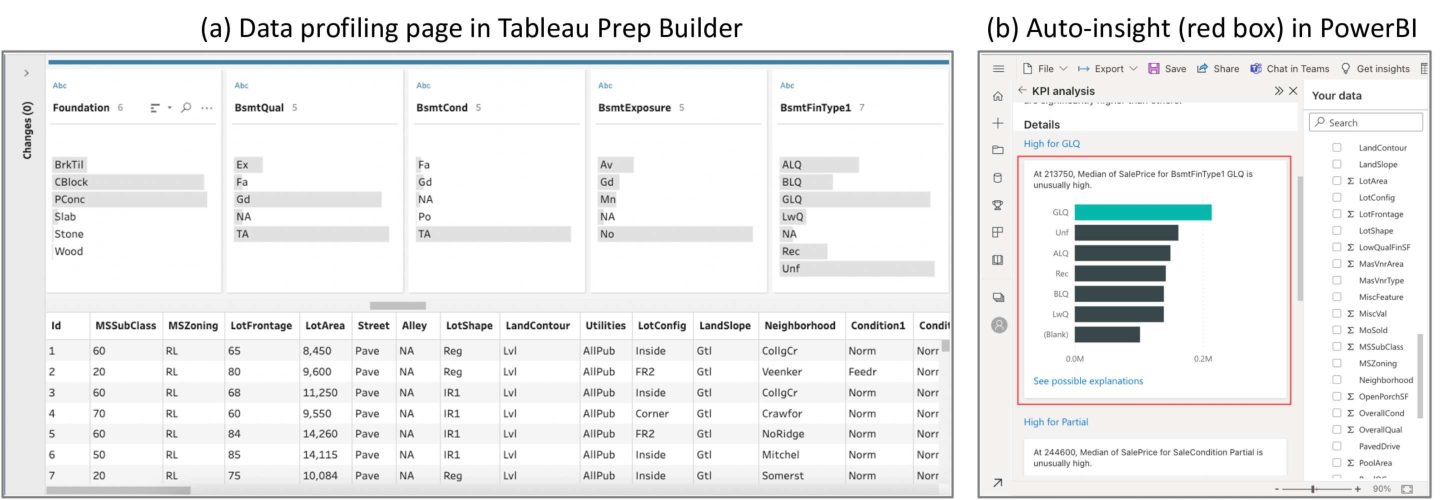
\includegraphics[width=1.0\textwidth]{figs/profiling-and-auto-insight.pdf}
\caption{Examples of Generating Initial Questions Using Tableau and PowerBI}
\label{fig:profiling-and-auto-insight}
\end{figure}


\stitle{Create Visualizations}
After getting some initial questions in mind, the next step is to create visualizations to answer the question. We create visualizations to examine the relationship between the `BsmtFinType1' column and the `SalePrice' column using Code and No Code interface. 

With the No Code interface, like in most commercial tools, a user can drag and drop column names into the visualization area to express the intention of creating a visualization on the specified column. For example, Figure \ref{fig:drag-drop-task-centric} (a) demonstrates how to use the drag and drop feature to create a visualization between `BsmtFinType1' and `SalePrice' using Tableau.

\begin{figure}[h]
\centering
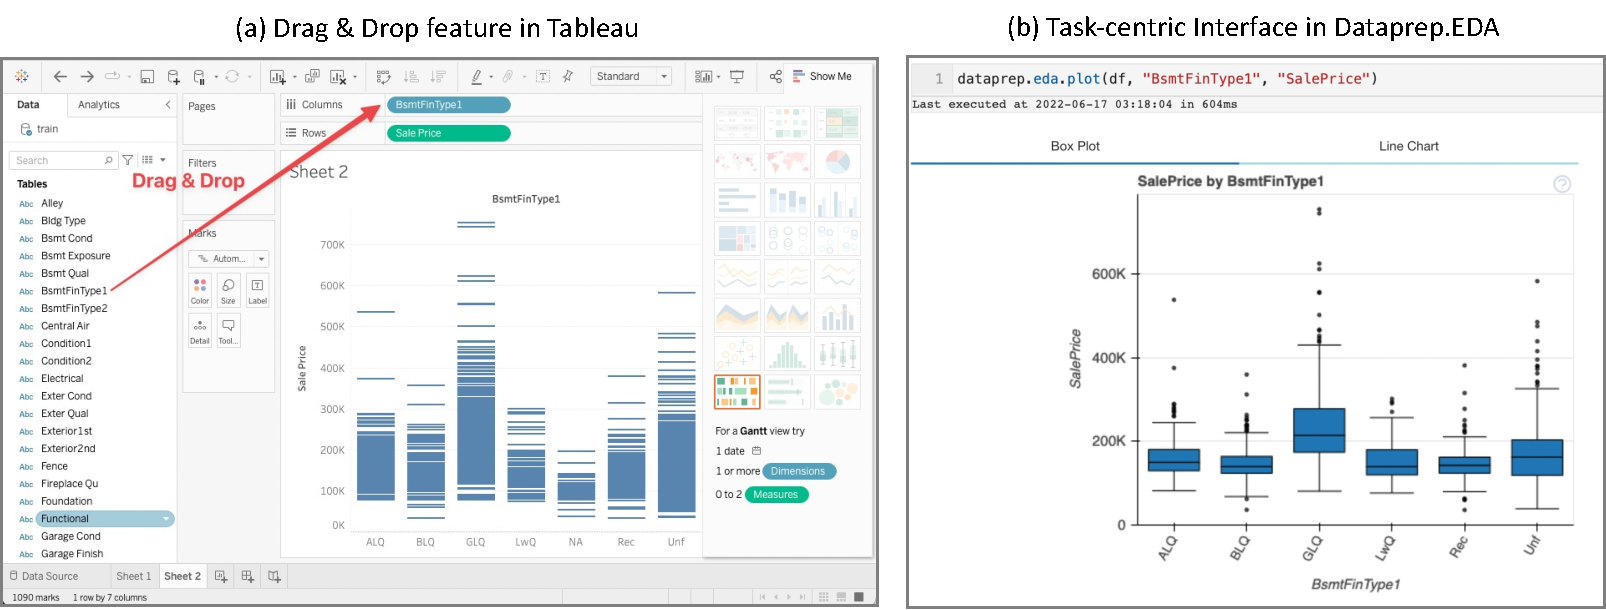
\includegraphics[width=\textwidth]{figs/drag-drop-task-centric.pdf}
\caption{Examples of Creating Visualizations Using Tableau and Dataprep.EDA}
\label{fig:drag-drop-task-centric}
\end{figure}



On the other hand, a Code interface requires a user to write several lines of code to accomplish the same goal. While this may seem more effortful, for an experienced user or effectively designed API the time required ought to be similar to that of an interactive one. Figure \ref{fig:drag-drop-task-centric} (b) demonstrates how to use the task-centric interface in DataPrep.EDA to create a visualization that helps complete the `understanding two variables' task.



\stitle{Examine Visualizations}
The Examining Visualizations stage then follows. The first step is directly inspecting the visualization to make sense of its visual scheme, identifying marks and visual features. From Figure \ref{fig:drag-drop-task-centric} (a) we can see that homes with `GLQ', which stands for `Good Living Quarters' have a tendency to have a higher price, which agrees with what we get from the auto-insights in Figure \ref{fig:profiling-and-auto-insight} (b). Moreover, we can also observe that there are a few extremely high sale price homes, which might be outliers. In this case, we can iterate with the question `are these high sale price GLQ homes outliers,' and go back to the `Create Visualizations' step. Such iteration is common in EDA practice.

Other EDA tools also allow users to do different interactions on the visualization. For example, Tableau (Figure \ref{fig:manual-interaction-auto-discovery} (a)) allows us to pick the outliers directly in the visualization and exclude it from the dataset if we do think the extraordinarily high sale price in the `GLQ' category is an outlier. Power BI can suggest other subgroups that make the distribution different. For example, in Figure \ref{fig:manual-interaction-auto-discovery} (b) Power BI indicates that homes with the `Foundation' equal to `BrkTil' (Brick Tile) have very few `GLQ'. The different ways to examine the visualization provided by the EDA tools help the user to come up with more questions, thus forming a `Generate Question - Create Visualizations - Examine Visualizations' cycle.


\begin{figure}[h]
\centering
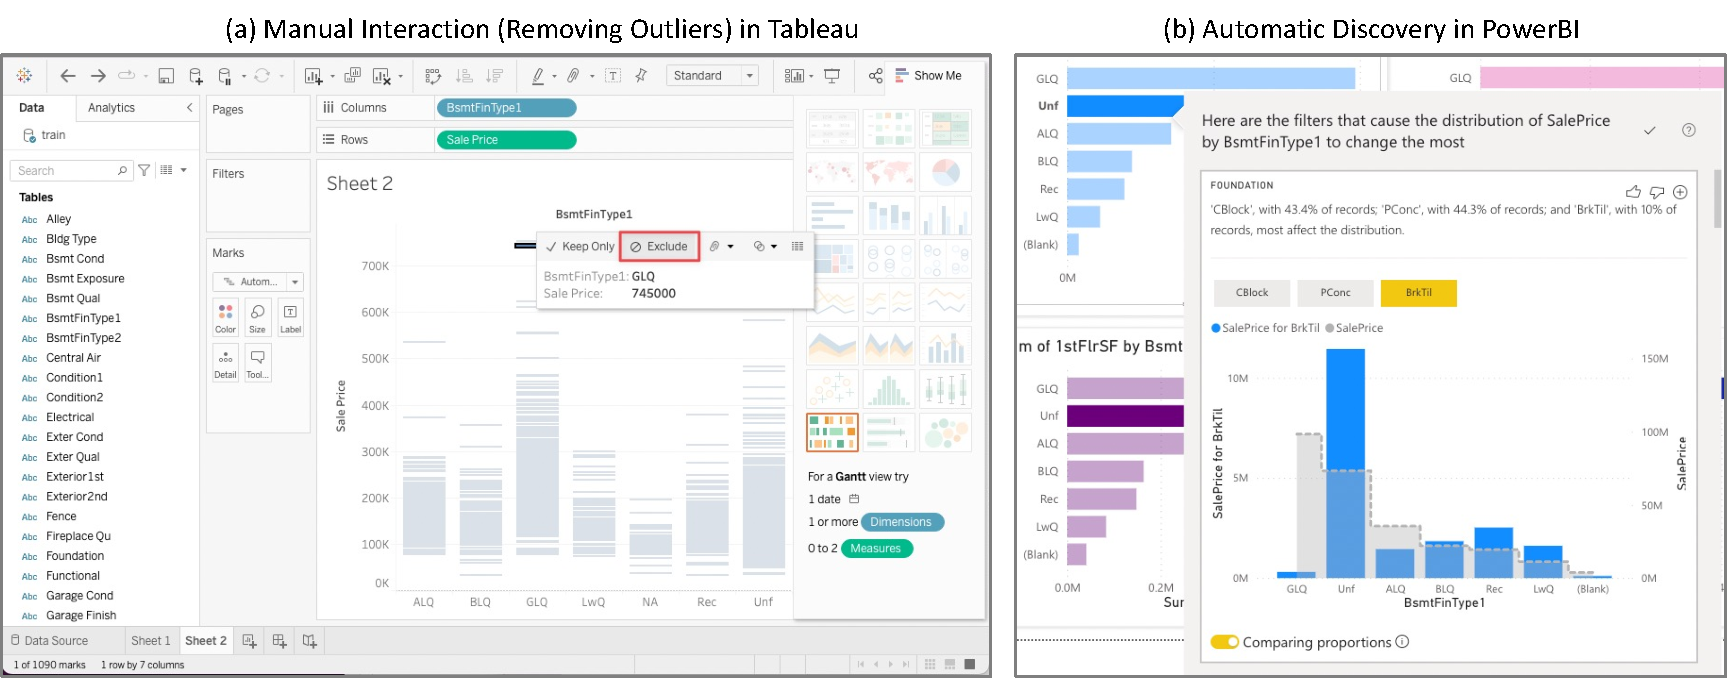
\includegraphics[width=\textwidth]{figs/manual-interaction-auto-discovery.pdf}
\caption{Examples of Examining Visualizations Using Tableau and PowerBI}
\label{fig:manual-interaction-auto-discovery}
\end{figure}





\section{Interfaces of EDA Tools}
\label{sec:feat}

Human interfaces, whether in the form of a programming API or interactive GUI, are an essential component of modern EDA tools. In this section, we outline the commonalities and differences among the surveyed tools and connect them to broader trends in EDA research. We do this with respect to the EDA stages described in the Introduction and outlined in Table~\ref{tab:feature}. We found from existing work and literature a common general pattern that users will go through interactively: generating initial questions, creating visualizations, and examining visualizations for answering initial questions or proposing new questions. We will discuss these stages separately in the following subsections. 



\begin{table}[t]
\caption{Interface Design of Commercial and Open-sourced EDA Tools}
\label{tab:feature}
\resizebox{\textwidth}{!}{%
\begin{tabular}{|ccc|c|c|c|c|c|c|c|c|c|c|c|}
\hline
\multicolumn{3}{|c|}{} & Tableau & Power BI & Viya & Looker & Quicksight & Superset & Voyage2 & Pandas & PandasPorfiling & DataPrep.EDA & Lux \\ \hline
\multicolumn{1}{|c|}{\multirow{7}{*}{Generate Initial Questions}} & \multicolumn{1}{c|}{\multirow{4}{*}{Data Profiling}} & Dataset Statistics & \checkmark & \checkmark & \checkmark  &  &  &  &  & \checkmark & \checkmark & \checkmark &  \\ \cline{3-14} 
\multicolumn{1}{|c|}{} & \multicolumn{1}{c|}{} & Univariate Distributions & \checkmark & \checkmark & \checkmark & \checkmark & \checkmark & \checkmark & \checkmark & \checkmark & \checkmark & \checkmark & \checkmark \\ \cline{3-14} 
\multicolumn{1}{|c|}{} & \multicolumn{1}{c|}{} & Multivariate Distributions & \checkmark & \checkmark & \checkmark & \checkmark & \checkmark & \checkmark & \checkmark & \checkmark & \checkmark & \checkmark & \checkmark \\ \cline{3-14} 
\multicolumn{1}{|c|}{} & \multicolumn{1}{c|}{} & Missing Value Overview & \checkmark & \checkmark & \checkmark &  &  &  &  & \checkmark & \checkmark & \checkmark &  \\ \cline{2-14} 
\multicolumn{1}{|c|}{} & \multicolumn{1}{c|}{\multirow{3}{*}{Auto-insight}} & Distribution & \checkmark & \checkmark & \checkmark  & & \checkmark  &  &  &  & \checkmark & \checkmark &  \\ \cline{3-14} 
\multicolumn{1}{|c|}{} & \multicolumn{1}{c|}{} & Anomalies & \checkmark  & \checkmark &  &  & \checkmark  &  &  &  &  &  &  \\ \cline{3-14} 
\multicolumn{1}{|c|}{} & \multicolumn{1}{c|}{} & Trend &  & \checkmark &  &  &  &  &  &  &  &  &  \\ \hline
\multicolumn{1}{|c|}{\multirow{7}{*}{Create Visualizations}} & \multicolumn{1}{c|}{\multirow{3}{*}{No Code}} & Template & \checkmark & \checkmark & \checkmark & \checkmark & \checkmark & \checkmark & \checkmark &  &  &  &  \\ \cline{3-14} 
\multicolumn{1}{|c|}{} & \multicolumn{1}{c|}{} & Drag \& Drop & \checkmark & \checkmark & \checkmark &  & \checkmark & \checkmark & \checkmark &  &  &  &  \\ \cline{3-14} 
\multicolumn{1}{|c|}{} & \multicolumn{1}{c|}{} & Natural Language & \checkmark & \checkmark &  &  & \checkmark &  &  &  &  &  &  \\ \cline{2-14} 
\multicolumn{1}{|c|}{} & \multicolumn{1}{c|}{\multirow{4}{*}{Code}} & Plot-centric & \checkmark & \checkmark & \checkmark & \checkmark & \checkmark & \checkmark &  & \checkmark &  &  &  \\ \cline{3-14} 
\multicolumn{1}{|c|}{} & \multicolumn{1}{c|}{} & Task-centric &  &  &  &  &  &  & \multicolumn{1}{l|}{} & \multicolumn{1}{l|}{} &  & \checkmark &  \\ \cline{3-14} 
\multicolumn{1}{|c|}{} & \multicolumn{1}{c|}{} & Profiling-centric &  &  &  &  &  &  & \multicolumn{1}{l|}{} & \multicolumn{1}{l|}{} & \checkmark &  &  \\ \cline{3-14} 
\multicolumn{1}{|c|}{} & \multicolumn{1}{c|}{} & Rec-centric &  &  &  &  &  &  & \checkmark &  &  &  & \checkmark \\ \hline
\multicolumn{1}{|c|}{\multirow{10}{*}{Examine Visualizations}} & \multicolumn{1}{c|}{\multirow{7}{*}{Manual Interaction}} & Select & \textbf{\checkmark} & \checkmark & \checkmark & \checkmark & \checkmark & \checkmark &  &  &  &  & \checkmark \\ \cline{3-14} 
\multicolumn{1}{|c|}{} & \multicolumn{1}{c|}{} & Explore & \checkmark & \checkmark & \checkmark & \checkmark & \checkmark & \checkmark & \checkmark &  &  &  &  \\ \cline{3-14} 
\multicolumn{1}{|c|}{} & \multicolumn{1}{c|}{} & Reconfigure & \checkmark & \checkmark &  & \checkmark & \checkmark & \checkmark & \checkmark &  &  &  &  \\ \cline{3-14} 
\multicolumn{1}{|c|}{} & \multicolumn{1}{c|}{} & Encode & \checkmark & \checkmark &  & \checkmark & \checkmark & \checkmark & \checkmark &  &  &  &  \\ \cline{3-14} 
\multicolumn{1}{|c|}{} & \multicolumn{1}{c|}{} & Abstract/Elaborate & \checkmark & \checkmark & \checkmark & \checkmark & \checkmark & \checkmark & \checkmark &  & \checkmark & \checkmark & \checkmark \\ \cline{3-14} 
\multicolumn{1}{|c|}{} & \multicolumn{1}{c|}{} & Filter & \checkmark & \checkmark & \checkmark & \checkmark & \checkmark & \checkmark & \checkmark &  &  &  &  \\ \cline{3-14} 
\multicolumn{1}{|c|}{} & \multicolumn{1}{c|}{} & Connect & \checkmark & \checkmark &  & \checkmark & \checkmark & \checkmark &  &  &  &  &  \\ \cline{2-14} 
\multicolumn{1}{|c|}{} & \multicolumn{1}{c|}{\multirow{3}{*}{Automatic Discovery}} & Auto-explanation &\checkmark  & \checkmark & \checkmark  &  &  &  &  &  &  &  &  \\ \cline{3-14} 
\multicolumn{1}{|c|}{} & \multicolumn{1}{c|}{} & Auto-insight & \checkmark & \checkmark &  &  & \checkmark &  &  &  &  &  &  \\ \cline{3-14} 
\multicolumn{1}{|c|}{} & \multicolumn{1}{c|}{} & Recommendation & \checkmark & \checkmark &  \checkmark &  &  &  & \checkmark  &  &  &  & \checkmark \\ \hline
\end{tabular}%
}
\end{table}






\subsection{Generate Initial Questions}
\label{sec:initial-question}

The first stage we will discuss concerns the generation of initial insights and hypotheses during EDA. As EDA's primary aim is to expose data through open-ended exploration \cite{tukey1977exploratory},
% \jrz{cite Tukey}\dqi{Cited} 
the first step of EDA is often to generate initial questions as starting points. We observed two approaches in our set of tools to generate the initial questions: data profiling and auto-insight. 


\stitle{Data Profiling} Traditionally, the starting point of exploratory data analysis is \emph{``overview first"}~\cite{DBLP:conf/vl/Shneiderman96}, which can be achieved by creating a data profiling report using tools like Pandas-Profiling~\cite{pandas-profiling} and DataPrep.EDA~\cite{DBLP:conf/sigmod/PengWLBYXCRW21}. There are several aspects of overview information in data profiling which we observe among our surveyed tools. The first aspect is providing summary statistics depicting the basic information of the dataset, such as the number of rows, the number of columns, the number of columns that contain missing values, and so on. The second aspect is providing distributional information like univariate distributions which depict the distribution of each column and multi-variate distributions which show the union distribution of multiple columns. And the final aspect is providing an overview for the distribution of missing values, such as the missing value percentage of each column and the missing value location distribution of each column. 

Data profiling often involves many potential avenues of exploration (and therefore tool affordances). Some of them may be useful and some of them may be redundant information. Thus, data profiling requires a degree of expertise if the interface does not provide obvious suggestions and hooks for the next steps. As many non-experts also need tools for profiling, there is great potential for future tools in automatically filtering useful information and providing inspiration. Auto-insight may be suitable for inspiring these non-experts for asking some questions with possible insights. 

\stitle{Auto Insight} While the profiling report provides a way for users to observe data and come up with some questions, commercial tools like PowerBI and open-source libraries like Dataprep.EDA provides another approach to start the exploration, automatically generating insights~\cite{DBLP:conf/sigmod/DingHXZZ19}, which may be more convenient for non-technical or time-sensitive users. The insights are detected by some predefined rules. If a visualization satisfies a rule, then an insight is reported. We identify three types of insights among our set of tools. The first type is detecting interesting distributions like highly skewed distributions or low-variance numerical columns. Also, detecting anomalies like outliers out of $3\sigma$ range is also an important type. The last type is detecting interesting trends in time series like periodic patterns or significant changes.


\subsection{Create Visualizations}\label{sec:create-vis}
After users have some questions in mind, the most common next stage in an EDA process is to investigate these questions more deeply. To accomplish this goal, the tools we examined offer means to create visualizations to probe the data about user questions and hypotheses. The means of creating visualizations can be divided into two types based on whether users need to write code: \emph{No Code} and \emph{Code}.

\stitle{No Code} The \emph{No Code} approaches provide a convenient way for non-technical users that are not familiar with programming languages to create visualizations. The first way is providing templates for users to fill out. According to the user-provided information like selected columns and visualization types in templates, the visualizations are automatically created. The second way is providing users with an interface to select the visible objects of interest \cite{drag-and-drop} like the columns and visualization types by dragging that used to create the visualization. If users want to change the selected visible objects, just drop them and switch to new ones. These visible objects can significantly save users' time by avoiding writing complex declarative languages or code. %\jrz{tableau, traditional office software, spotfire? -- cite old Jock Mackinlay paper to show foundations of drag and drop work}. \dqi{Added \cite{drag-and-drop}}
The third way is providing users natural language interface~\cite{DBLP:conf/uist/SetlurBTGC16} including natural language text and speech~\cite{speech-to-vis}, which allows users directly input a question using natural language and then recommend the most related visualizations to answer this question. The learning curve for these tools is thus much reduced, assuming recommendations are of high accuracy and users can adequately describe their interests \cite{nlpSurvey}.


\begin{figure}[t]
    \centering
    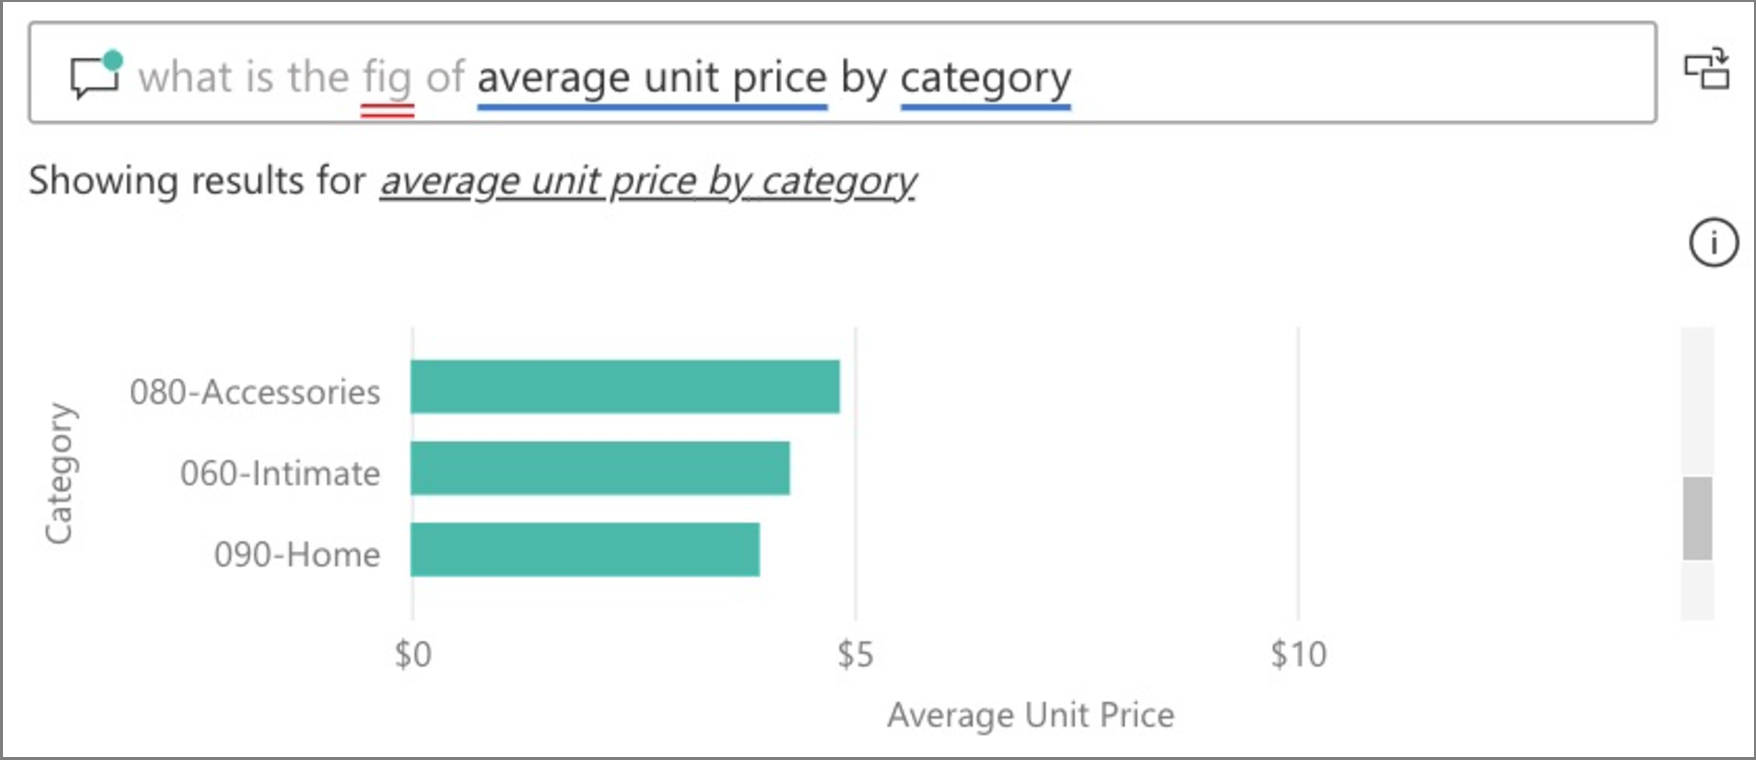
\includegraphics[width=.8\textwidth]{figs/ask-question.pdf}
    \caption{An example of the asking question feature (the Q\&A in Power BI)}
    \label{fig:ask-question}
\end{figure}


\stitle{Code}
While \emph{No Code} approaches may be more convenient for non-technical users, their interfaces may be less flexible for advanced users. For this reason, EDA tools also often offer \emph{Code} interfaces which provide analysts with more complex and adjustable tools (albeit with higher complexity and training requirements). Based on the granularity of the API, the \emph{Code} interface has four common types that we have observed: \emph{Plotting-Centric}, \emph{Recommendation-Centric}, \emph{Profiling-Centric} and \emph{Task-Centric}. \emph{Plot-Centric} interfaces provide APIs which are used to create a specific type of visualization. For example, the \texttt{plot.hist} in Pandas is used to create histograms, and the \texttt{plot.bar} is used to create bar charts. \emph{Recommendation-Centric} interfaces provide APIs which can give users recommendations according to the input datasets. However, the recommendation strategies are often in one manner. For example, Lux~\cite{DBLP:journals/pvldb/LeeTABCKMSYHP21} automatically recommends bivariate correlation, univariate distribution and occurrence. \emph{Profiling-Centric} interfaces provide APIs which can produce multiple visualizations with one manner for all datasets. \emph{Task-Centric} interfaces provide declarative APIs which are create all the visualizations required by a specific EDA task. For example, DataPrep.EDA~\cite{DBLP:conf/sigmod/PengWLBYXCRW21} provides APIs for statistical modeling tasks. If users want to create visualizations about missing values, just call \texttt{plot\_missing} in Dataprep.EDA. Compared to plotting-centric interfaces which are under a grain granularity and profiling-centric interfaces which are under a coarse granularity, task-centric interfaces leverage a trade-off of visualization granularity. Also, task-centric interfaces are easy to customize, e.g. adjusting bin sizes when plotting bar charts for a specific EDA task.




\subsection{Examine Visualizations}
After visualizations are created, the last step is to examine the visualizations. The goal is to answer initial questions and find something interesting for proposing new questions. To examine the visualizations, one can manually interact with the created visualizations to develop an understanding. The system itself can also examine visualizations by automatically discovering possible insights and explanations, and providing recommendations. Hence, we classify the interface of examining visualizations into two categories: \emph{manual interaction} and \emph{automatic discovery}.


\stitle{Examination with Manual Interaction}
There exist many works that summarize the interactions for examining visualizations from different perspectives. We leverage the classification in a survey~\cite{DBLP:journals/tvcg/YiKSJ07}. As shown in Table~\ref{tab:feature} (more specifically, \emph{Examine Visualizations --- Manual Interaction}), it classifies the interactions into seven types. Users often choose the \emph{select} interaction to highlight their most interesting items in created visualizations. The way of highlighting can be a color change, or an increase of the shape size. In the other way, users can employ the \emph{explore} interaction to explore a different collection of items. One example is panning the map. The \emph{reconfigure} interaction allows users to change the \emph{``spatial arrangement of representations"}~\cite{DBLP:journals/tvcg/YiKSJ07} in a visualization, e.g. when users want to sort bar charts according to the heights of bars, the sorting operation rearranges the bars. The \emph{encode} interaction can change the representation of the visualizations, such as changing the bar chart to pie chart, and changing the color and shape of each item. The \emph{Abstract/Elaborate} interaction allows the user to see more or fewer details, such as zooming-in for more details and zooming-out for less details (more overviews). The \emph{filter} interaction can change the data used for visualization by only keeping items satisfying some conditions. For example, if the users are interested in the subset of data with condition \texttt{age < 20}, they can add a filter \texttt{age < 20} to visualize this subset. The \emph{connect} interaction is used to highlight corresponding parts among multiple visualizations for selected items. When different visualizations are created for the same dataset, the user can select one item from one visualization, and the \emph{connect} interaction can highlight the corresponding parts related to the selected item in other visualizations. 

\stitle{Examination with Automatic Discovery}
Apart from manual interaction to examine the visualizations, the system can automatically discover interesting insights and possible explanations to some questions, which helps users to examine whether the created visualizations can answer their initial questions. Three ways of automatic discovery are summarized from our set of tools. The first way is also called \emph{auto-insight}. Compared to the \emph{auto-insight} mentioned in Section~\ref{sec:initial-question} which detects the insights over the full data, the \emph{auto-insight} here just focuses on the data leveraged by created visualizations, i.e. subsets of data. These insights may help users to answer initial questions and propose new questions. The second way is called \emph{auto-explanation}, which can automatically generate possible explanations for interesting aspects in created visualizations. These explanations may answer initial questions and inspire further questions. The third way is called \emph{recommendation}. Apart from the created visualizations, some systems can also recommend related visualizations by changing elements in current visualizations, which may be helpful to find the answer for initial questions or generate further questions. For example, Lux~\cite{DBLP:journals/pvldb/LeeTABCKMSYHP21} can automatically recommend related visualizations by making some changes to existing visualizations (e.g., add an additional attribute, add a filter or remove an attribute), which provides users answers and inspirations with external information.


\section{Discussion}
\label{sec:discussion}

In this section, we discuss the current status of interfaces for commercial and open-source EDA tools on different stages, and identify possible research opportunities.


\subsection{Generate Initial Questions}

\stitle{Profiling for dependency relationships} We observed most tools only provide profiling for basic statistics of a single column and at most two columns. However, it lacks the support of more complex profiling such as inclusion dependency and functional dependency, which are widely studied in the database community. This limits the insights that users can observe from the profiling result. The challenge here is how to support more complex profiling and make the process efficient. For example, some approximate approaches can be used. For more types of profiling and more discussions on this topic, we refer interested readers to a data profiling survey~\cite{DBLP:journals/vldb/AbedjanGN15}. 


\stitle{From descriptive insights to prescriptive insights} We observed the insights provided by most tools are descriptive (e.g., a group-by query has a very large group), while the research community has many studies on prescriptive insights~\cite{DBLP:journals/pvldb/0002M13, DBLP:conf/sigmod/BailisGMNRS17, DBLP:journals/corr/abs-2102-05308} (e.g., explaining why the group size is too large). We 
have seen the trend of supporting these prescriptive insights in EDA tools. For example, Tableau's ``Explain Data'' feature  gives possible explanations for unexpected aggregate values, such as "why is the average housing price too high?".

\stitle{Seamlessly integrate profiling and auto-insight} Profiling and auto-insight have their own advantages and limitations. For profiling, it creates many visualizations that cover the basic data characteristics of all columns. However, users may need to check a lot of visualizations until they find something interesting. For auto-insight, it directly reports the visualizations that users may be interested in, thus they can spend less time finding something interesting. However, it may not align with users' real interests or cover all the columns (e.g., users are interested in column A, but none of the returned insights contains column A). 

Given the pros and cons of profiling and auto-insight interfaces, one natural question is whether we can combine them to better serve users. For example, if the profiling report contains too many visualizations, then the auto-insight feature can help highlight possible interesting visualizations and prioritize them to users. Furthermore, one can also add an auto-insight section in the report, helping users automatically discover questions that are not covered by observing the report. For this approach, the auto-insight and report should be treated as a whole and the search space of insight should be reconsidered, e.g., by excluding the insight that can be found using other visualizations in the report.



\subsection{Create Visualizations}

\stitle{Combining Code and No Code interfaces} The No Code interface is easy to use and has fewer requirements (no programming skill is needed). However, it lacks transparency and users have limited control of the creation process. On the other hand, the Code interface provides a more flexible way to create visualizations, but it is not accessible to non-programmers. 

To make the Code interface easier to use, we observed that there is a trend of adding GUI and interaction in the coding environment like Jupyter Notebook~\cite{DBLP:conf/chi/KeryRWHP20, DBLP:journals/tvcg/AlspaughZLJH19}. For example, DataPrep.EDA~\cite{DBLP:conf/sigmod/PengWLBYXCRW21} and Lux~\cite{DBLP:journals/pvldb/LeeTABCKMSYHP21} generate interactive visualizations, and Bamboolib~\cite{bamboolib}, PandasGUI~\cite{pandasgui} and Mage~\cite{DBLP:conf/uist/KeryRHMWP20} provide GUIs for data exploration. By integrating Code with Notebook GUI, the Code interface is not only flexible but also easy to use. To increase the transparency of the No Code interface, one idea is to automatically generate the code for each visualization such that users can copy and paste the code to a programming environment and reproduce the visualization. In this way, users have more flexibility to customize visualizations using a programming language.


\stitle{Natural language as a unified interface} The No Code interface such as drag \& drop is convenient to create visualizations, especially for non-technical users. The advanced feature such as supporting natural language interfaces takes one step further. It allows users who are not even familiar with BI tools to create visualizations. The current support of natural language interfaces is still limited. As shown in Figure~\ref{fig:ask-question}, the supported questions are relatively simple and follow certain patterns. If a question is not supported, it may recommend the closest question to the user's input. For example, the gray keywords are not understood by the system, thus it suggests a close question and shows its result. 

Although natural language support is at an early stage, it has the potential to become a unified interface for EDA. For example, users may first ask ``what's interesting about data" to discover insights and get some initial questions. Then the system returns an insight that the average salary in Beijing is much lower than in other cities. After that, the user asks ``why the average salary is low?" through the natural language interface. Finally the system receives the question and gives an explanation. There are many challenges that exist to build such a system. For example, handling the ambiguity of natural language queries, mapping the query to visual representation and managing the dialogue system~\cite{nlpSurvey}. We refer interested readers to a recent survey for more discussion~\cite{nlpSurvey}.





\subsection{Examine Visualizations}

\stitle{Augmented Analytics} One big trend of data analysis is the engagement of artificial intelligence (AI) techniques. Gartner uses the term ``augmented analytics" to represent the approach \emph{``that automates insights using machine learning and natural-language generation"}, and shows that it \emph{``marks the next wave of disruption in the data and analytics market"}~\cite{sallam2017augmented}. As discussed in Section~\ref{sec:feat}, the AI techniques can help at each stage, such as automatically recommending insights to start exploration, providing a natural language interface for creating visualizations, and automatically discovering interesting insights and giving possible explanations to understand visualizations. Although AI techniques are powerful, there still exist some challenges when applying them in EDA scenarios. For example, EDA is a time-sensitive process, thus the efficiency of applying AI techniques could be a concern, especially for a large dataset. Then the question is how to make AI techniques efficient for this situation. There exist some opportunities when we consider the property of EDA scenarios. For example, EDA is a human-in-the-loop process, and AI techniques should be applied to better serve humans. Hence, some decisions can be proposed to humans (e.g., selecting the analyzed variables), rather than computing all possibilities. This can help reduce computing time and improve user experience. Besides, when users make a decision, the thinking time can also be leveraged for computation~\cite{DBLP:conf/sigmod/CrottyGZBK16}.

Apart from the efficiency issues, there are some other practical issues of AI models~\cite{poursabzi2021manipulating, kaur2020interpreting}. For example, the model is trained on training data, but the data itself may be biased. In this case, the model may guide users in a wrong way, and finally lead to a wrong conclusion. For example,  Amazon previously used the recruitment system to decide whether to recruit a candidate or not, which proves to have considered some sensitive factors~\cite{yan2020silva}. For more discussion about how AI can help automate the EDA system, we refer interested readers to a recent survey~\cite{DBLP:conf/sigmod/MiloS20}.


\stitle{Leverage context information} While the discussed systems can automatically discover insights and explanations, the context information is not well leveraged. In the following, we discuss how two types of context, data context and session context, may help improve the automatic discovery process.

\underline{Data Context.} The data itself has semantic meanings and is helpful for multiple tasks, such as data integration, data discovery, and automatic data preparation~\cite{DBLP:conf/cidr/HulsebosGGDGD22}. However, we found this is not well used in the studied tools. For example, one type of auto-insight is to aggregate numerical columns in each group and see whether one group has a much larger size than the others. In practice, some aggregations may be meaningless, such as computing the sum of age. If data context is considered, this kind of insight will not be shown to confuse users. 

\underline{Session Context.} As EDA is an iterative process, some discoveries from users might be reused, which can reduce redundant steps in EDA. For example, if an insight is already reported in the last few steps, then it can be regarded as a known fact to users and its weight for ranking can be reduced. Besides, the computation from previous steps may be reused, such that the efficiency can be improved~\cite{DBLP:conf/sigmod/CrottyGZBK16}. 






\begin{thebibliography}{10}
\itemsep=1pt
\begin{small}
\bibitem{bamboolib}
Bamboolib.
\newblock https://bamboolib.8080labs.com/. Date accessed: 2022-06-07.

\bibitem{pandas-profiling}
Pandas-profiling.
\newblock https://github.com/ydataai/pandas-profiling. Date accessed:
  2022-06-07.

\bibitem{pandasgui}
Pandasgui.
\newblock https://github.com/adamerose/PandasGUI. Date accessed: 2022-06-07.

\bibitem{DBLP:journals/vldb/AbedjanGN15}
Z.~Abedjan, L.~Golab, and F.~Naumann.
\newblock Profiling relational data: a survey.
\newblock {\em {VLDB} J.}, 24(4):557--581, 2015.

\bibitem{DBLP:journals/tvcg/AlspaughZLJH19}
S.~Alspaugh, N.~Zokaei, A.~Liu, C.~Jin, and M.~A. Hearst.
\newblock Futzing and moseying: Interviews with professional data analysts on
  exploration practices.
\newblock {\em {IEEE} Trans. Vis. Comput. Graph.}, 25(1):22--31, 2019.

\bibitem{quicksight}
{Amazon Web Services, Inc.}
\newblock Amazon quicksight: The most popular cloud-native, serverless bi
  service.
\newblock {https://aws.amazon.com/quicksight. Date accessed: 2022-06-20}.

\bibitem{superset}
{Apache Software Foundation}.
\newblock Apache superset: A modern, enterprise-ready business intelligence web
  application.
\newblock {https://github.com/apache/superset. Date accessed: 2022-06-20}.

\bibitem{DBLP:conf/sigmod/BailisGMNRS17}
P.~Bailis, E.~Gan, S.~Madden, D.~Narayanan, K.~Rong, and S.~Suri.
\newblock Macrobase: Prioritizing attention in fast data.
\newblock In S.~Salihoglu, W.~Zhou, R.~Chirkova, J.~Yang, and D.~Suciu,
  editors, {\em Proceedings of the 2017 {ACM} International Conference on
  Management of Data, {SIGMOD} Conference 2017, Chicago, IL, USA, May 14-19,
  2017}, pages 541--556. {ACM}, 2017.

\bibitem{DBLP:journals/cgf/BattleH19}
L.~Battle and J.~Heer.
\newblock Characterizing exploratory visual analysis: {A} literature review and
  evaluation of analytic provenance in tableau.
\newblock {\em Comput. Graph. Forum}, 38(3):145--159, 2019.

\bibitem{ames}
D.~D. Cock.
\newblock Ames, iowa: Alternative to the boston housing data as an end of
  semester regression project.
\newblock {\em Journal of Statistics Education}, 19(3):null, 2011.

\bibitem{powerbi}
M.~Corporation.
\newblock Microsoft power bi.
\newblock {https://powerbi.microsoft.com/. Date accessed: 2022-06-20}.

\bibitem{DBLP:conf/sigmod/CrottyGZBK16}
A.~Crotty, A.~Galakatos, E.~Zgraggen, C.~Binnig, and T.~Kraska.
\newblock The case for interactive data exploration accelerators (ideas).
\newblock In C.~Binnig, A.~D. Fekete, and A.~Nandi, editors, {\em Proceedings
  of the Workshop on Human-In-the-Loop Data Analytics, HILDA@SIGMOD 2016, San
  Francisco, CA, USA, June 26 - July 01, 2016}, page~11. {ACM}, 2016.

\bibitem{DBLP:journals/ivs/CuiBYE19}
Z.~Cui, S.~K. Badam, M.~A. Yal{\c{c}}in, and N.~Elmqvist.
\newblock Datasite: Proactive visual data exploration with computation of
  insight-based recommendations.
\newblock {\em Inf. Vis.}, 18(2), 2019.

\bibitem{DBLP:conf/sigmod/DingHXZZ19}
R.~Ding, S.~Han, Y.~Xu, H.~Zhang, and D.~Zhang.
\newblock Quickinsights: Quick and automatic discovery of insights from
  multi-dimensional data.
\newblock In P.~A. Boncz, S.~Manegold, A.~Ailamaki, A.~Deshpande, and
  T.~Kraska, editors, {\em Proceedings of the 2019 International Conference on
  Management of Data, {SIGMOD} Conference 2019, Amsterdam, The Netherlands,
  June 30 - July 5, 2019}, pages 317--332. {ACM}, 2019.

\bibitem{gartner}
{\relax Gartner Inc.}
\newblock Gartner magic quadrant for analytics and business intelligence
  platforms.
\newblock https://www.gartner.com/en/documents/3996944. Date accessed:
  2022-06-07.

\bibitem{DBLP:journals/vi/GhoshNMQM18}
A.~Ghosh, M.~Nashaat, J.~Miller, S.~Quader, and C.~Marston.
\newblock A comprehensive review of tools for exploratory analysis of tabular
  industrial datasets.
\newblock {\em Vis. Informatics}, 2(4):235--253, 2018.

\bibitem{looker}
{Google LLC}.
\newblock Looker \& google cloud.
\newblock {https://www.looker.com/google-cloud/. Date accessed: 2022-06-20}.

\bibitem{DBLP:journals/cacm/HeerS12}
J.~Heer and B.~Shneiderman.
\newblock Interactive dynamics for visual analysis.
\newblock {\em Commun. {ACM}}, 55(4):45--54, 2012.

\bibitem{DBLP:conf/cidr/HulsebosGGDGD22}
M.~Hulsebos, S.~Gathani, J.~Gale, I.~Dillig, P.~Groth, and {\c{C}}.~Demiralp.
\newblock Making table understanding work in practice.
\newblock In {\em 12th Conference on Innovative Data Systems Research, {CIDR}
  2022, Chaminade, CA, USA, January 9-12, 2022}. www.cidrdb.org, 2022.

\bibitem{kaur2020interpreting}
H.~Kaur, H.~Nori, S.~Jenkins, R.~Caruana, H.~Wallach, and J.~Wortman~Vaughan.
\newblock Interpreting interpretability: understanding data scientists' use of
  interpretability tools for machine learning.
\newblock In {\em Proceedings of the 2020 CHI conference on human factors in
  computing systems}, pages 1--14, 2020.

\bibitem{DBLP:conf/uist/KeryRHMWP20}
M.~B. Kery, D.~Ren, F.~Hohman, D.~Moritz, K.~Wongsuphasawat, and K.~Patel.
\newblock mage: Fluid moves between code and graphical work in computational
  notebooks.
\newblock In S.~T. Iqbal, K.~E. MacLean, F.~Chevalier, and S.~Mueller, editors,
  {\em {UIST} '20: The 33rd Annual {ACM} Symposium on User Interface Software
  and Technology, Virtual Event, USA, October 20-23, 2020}, pages 140--151.
  {ACM}, 2020.

\bibitem{DBLP:conf/chi/KeryRWHP20}
M.~B. Kery, D.~Ren, K.~Wongsuphasawat, F.~Hohman, and K.~Patel.
\newblock The future of notebook programming is fluid.
\newblock In R.~Bernhaupt, F.~F. Mueller, D.~Verweij, J.~Andres, J.~McGrenere,
  A.~Cockburn, I.~Avellino, A.~Goguey, P.~Bj{\o}n, S.~Zhao, B.~P. Samson, and
  R.~Kocielnik, editors, {\em Extended Abstracts of the 2020 {CHI} Conference
  on Human Factors in Computing Systems, {CHI} 2020, Honolulu, HI, USA, April
  25-30, 2020}, pages 1--8. {ACM}, 2020.

\bibitem{DBLP:journals/pvldb/Kraska18}
T.~Kraska.
\newblock Northstar: An interactive data science system.
\newblock {\em Proc. {VLDB} Endow.}, 11(12):2150--2164, 2018.

\bibitem{DBLP:journals/pvldb/LeeTABCKMSYHP21}
D.~J.~L. Lee, D.~Tang, K.~Agarwal, T.~Boonmark, C.~Chen, J.~Kang,
  U.~Mukhopadhyay, J.~Song, M.~Yong, M.~A. Hearst, and A.~G. Parameswaran.
\newblock Lux: Always-on visualization recommendations for exploratory
  dataframe workflows.
\newblock {\em Proc. {VLDB} Endow.}, 15(3):727--738, 2021.

\bibitem{DBLP:journals/corr/abs-2102-05308}
B.~Lockhart, J.~Peng, W.~Wu, J.~Wang, and E.~Wu.
\newblock Explaining inference queries with bayesian optimization.
\newblock {\em CoRR}, abs/2102.05308, 2021.

\bibitem{DBLP:conf/icde/LuoQ0018}
Y.~Luo, X.~Qin, N.~Tang, and G.~Li.
\newblock Deepeye: Towards automatic data visualization.
\newblock In {\em 34th {IEEE} International Conference on Data Engineering,
  {ICDE} 2018, Paris, France, April 16-19, 2018}, pages 101--112. {IEEE}
  Computer Society, 2018.

\bibitem{martinez2017exploratory}
W.~L. Martinez, A.~R. Martinez, and J.~L. Solka.
\newblock {\em Exploratory data analysis with MATLAB{\textregistered}}.
\newblock Chapman and Hall/CRC, 2017.

\bibitem{DBLP:conf/sigmod/MiloS20}
T.~Milo and A.~Somech.
\newblock Automating exploratory data analysis via machine learning: An
  overview.
\newblock In D.~Maier, R.~Pottinger, A.~Doan, W.~Tan, A.~Alawini, and H.~Q.
  Ngo, editors, {\em Proceedings of the 2020 International Conference on
  Management of Data, {SIGMOD} Conference 2020, online conference [Portland,
  OR, USA], June 14-19, 2020}, pages 2617--2622. {ACM}, 2020.

\bibitem{reback2020pandas}
T.~pandas~development team.
\newblock pandas-dev/pandas: Pandas.
\newblock Feb. 2020.

\bibitem{DBLP:conf/qrs/PapamichailDS16}
M.~Papamichail, T.~G. Diamantopoulos, and A.~L. Symeonidis.
\newblock User-perceived source code quality estimation based on static
  analysis metrics.
\newblock In {\em 2016 {IEEE} International Conference on Software Quality,
  Reliability and Security, {QRS} 2016, Vienna, Austria, August 1-3, 2016},
  pages 100--107. {IEEE}, 2016.

\bibitem{DBLP:conf/sigmod/PengWLBYXCRW21}
J.~Peng, W.~Wu, B.~Lockhart, S.~Bian, J.~N. Yan, L.~Xu, Z.~Chi, J.~M.
  Rzeszotarski, and J.~Wang.
\newblock Dataprep.eda: Task-centric exploratory data analysis for statistical
  modeling in python.
\newblock In G.~Li, Z.~Li, S.~Idreos, and D.~Srivastava, editors, {\em {SIGMOD}
  '21: International Conference on Management of Data, Virtual Event, China,
  June 20-25, 2021}, pages 2271--2280. {ACM}, 2021.

\bibitem{kdnuggets}
G.~Piatetsky.
\newblock Python leads the 11 top data science, machine learning platforms:
  Trends and analysis.
\newblock
  {https://www.kdnuggets.com/2019/05/poll-top-data-science-machine-learning-platforms.html.
  Date accessed: 2022-06-07}.

\bibitem{poursabzi2021manipulating}
F.~Poursabzi-Sangdeh, D.~G. Goldstein, J.~M. Hofman, J.~W. Wortman~Vaughan, and
  H.~Wallach.
\newblock Manipulating and measuring model interpretability.
\newblock In {\em Proceedings of the 2021 CHI conference on human factors in
  computing systems}, pages 1--52, 2021.

\bibitem{sallam2017augmented}
R.~Sallam, C.~Howson, and C.~J. Idoine.
\newblock Augmented analytics is the future of data and analytics.
\newblock {\em Gartner, Inc}, 27, 2017.

\bibitem{viya}
{SAS Institute Inc.}
\newblock Sas viya: Confident decisions at every moment.
\newblock {https://www.sas.com/en\_ca/software/viya.html. Date accessed:
  2022-06-20}.

\bibitem{DBLP:conf/uist/SetlurBTGC16}
V.~Setlur, S.~E. Battersby, M.~Tory, R.~Gossweiler, and A.~X. Chang.
\newblock Eviza: {A} natural language interface for visual analysis.
\newblock In J.~Rekimoto, T.~Igarashi, J.~O. Wobbrock, and D.~Avrahami,
  editors, {\em Proceedings of the 29th Annual Symposium on User Interface
  Software and Technology, {UIST} 2016, Tokyo, Japan, October 16-19, 2016},
  pages 365--377. {ACM}, 2016.

\bibitem{nlpSurvey}
L.~Shen, E.~Shen, Y.~Luo, X.~Yang, X.~Hu, X.~Zhang, Z.~Tai, and J.~Wang.
\newblock Towards natural language interfaces for data visualization: A survey.
\newblock {\em arXiv preprint arXiv:2109.03506}, 2021.

\bibitem{DBLP:conf/vl/Shneiderman96}
B.~Shneiderman.
\newblock The eyes have it: {A} task by data type taxonomy for information
  visualizations.
\newblock In {\em Proceedings of the 1996 {IEEE} Symposium on Visual Languages,
  Boulder, Colorado, USA, September 3-6, 1996}, pages 336--343. {IEEE} Computer
  Society, 1996.

\bibitem{DBLP:journals/pvldb/SiddiquiKLKP16}
T.~Siddiqui, A.~Kim, J.~Lee, K.~Karahalios, and A.~G. Parameswaran.
\newblock Effortless data exploration with zenvisage: An expressive and
  interactive visual analytics system.
\newblock {\em Proc. {VLDB} Endow.}, 10(4):457--468, 2016.

\bibitem{DBLP:journals/rjour/StaniakB19}
M.~Staniak and P.~Biecek.
\newblock The landscape of {R} packages for automated exploratory data
  analysis.
\newblock {\em R J.}, 11(2):347, 2019.

\bibitem{DBLP:journals/tvcg/StolteTH02}
C.~Stolte, D.~Tang, and P.~Hanrahan.
\newblock Polaris: {A} system for query, analysis, and visualization of
  multidimensional relational databases.
\newblock {\em {IEEE} Trans. Vis. Comput. Graph.}, 8(1):52--65, 2002.

\bibitem{tableau}
{TABLEAU SOFTWARE, LLC}.
\newblock Tableau.
\newblock {https://www.tableau.com/. Date accessed: 2022-06-20}.

\bibitem{speech-to-vis}
J.~Tang, Y.~Luo, M.~Ouzzani, G.~Li, and H.~Chen.
\newblock Sevi: Speech-to-visualization through neural machine translation.
\newblock In Z.~Ives, A.~Bonifati, and A.~E. Abbadi, editors, {\em {SIGMOD}
  '22: International Conference on Management of Data, Philadelphia, PA, USA,
  June 12 - 17, 2022}, pages 2353--2356. {ACM}, 2022.

\bibitem{tiobe}
{\relax TIOBE Software BV}.
\newblock Tiobe index.
\newblock https://www.tiobe.com/tiobe-index/. Date accessed: 2022-06-07.

\bibitem{tukey1977exploratory}
J.~W. Tukey et~al.
\newblock {\em Exploratory data analysis}, volume~2.
\newblock Reading, MA, 1977.

\bibitem{DBLP:journals/jossw/VanderPlasGHMWS18}
J.~VanderPlas, B.~E. Granger, J.~Heer, D.~Moritz, K.~Wongsuphasawat,
  A.~Satyanarayan, E.~Lees, I.~Timofeev, B.~Welsh, and S.~Sievert.
\newblock Altair: Interactive statistical visualizations for python.
\newblock {\em J. Open Source Softw.}, 3(32):1057, 2018.

\bibitem{DBLP:journals/pvldb/VartakRMPP15}
M.~Vartak, S.~Rahman, S.~Madden, A.~G. Parameswaran, and N.~Polyzotis.
\newblock {SEEDB:} efficient data-driven visualization recommendations to
  support visual analytics.
\newblock {\em Proc. {VLDB} Endow.}, 8(13):2182--2193, 2015.

\bibitem{drag-and-drop}
A.~Whilden, D.~Karis, V.~Setlur, R.~Degtyar, J.~Que, and F.~Lymperopoulos.
\newblock Blocks: Creating rich tables with drag-and-drop interaction.
\newblock 2022.

\bibitem{DBLP:journals/corr/abs-1911-00568}
K.~Wongsuphasawat, Y.~Liu, and J.~Heer.
\newblock Goals, process, and challenges of exploratory data analysis: An
  interview study.
\newblock {\em CoRR}, abs/1911.00568, 2019.

\bibitem{DBLP:conf/chi/WongsuphasawatQ17}
K.~Wongsuphasawat, Z.~Qu, D.~Moritz, R.~Chang, F.~Ouk, A.~Anand, J.~D.
  Mackinlay, B.~Howe, and J.~Heer.
\newblock Voyager 2: Augmenting visual analysis with partial view
  specifications.
\newblock In G.~Mark, S.~R. Fussell, C.~Lampe, m.~c. schraefel, J.~P. Hourcade,
  C.~Appert, and D.~Wigdor, editors, {\em Proceedings of the 2017 {CHI}
  Conference on Human Factors in Computing Systems, Denver, CO, USA, May 06-11,
  2017}, pages 2648--2659. {ACM}, 2017.

\bibitem{DBLP:journals/pvldb/0002M13}
E.~Wu and S.~Madden.
\newblock Scorpion: Explaining away outliers in aggregate queries.
\newblock {\em Proc. {VLDB} Endow.}, 6(8):553--564, 2013.

\bibitem{DBLP:conf/cidr/WuPMZR17}
E.~Wu, F.~Psallidas, Z.~Miao, H.~Zhang, and L.~Rettig.
\newblock Combining design and performance in a data visualization management
  system.
\newblock In {\em 8th Biennial Conference on Innovative Data Systems Research,
  {CIDR} 2017, Chaminade, CA, USA, January 8-11, 2017, Online Proceedings}.
  www.cidrdb.org, 2017.

\bibitem{yan2020silva}
J.~N. Yan, Z.~Gu, H.~Lin, and J.~M. Rzeszotarski.
\newblock Silva: Interactively assessing machine learning fairness using
  causality.
\newblock In {\em Proceedings of the 2020 CHI conference on human factors in
  computing systems}, pages 1--13, 2020.

\bibitem{yan2021tessera}
J.~N. Yan, Z.~Gu, and J.~M. Rzeszotarski.
\newblock Tessera: Discretizing data analysis workflows on a task level.
\newblock In {\em Proceedings of the 2021 CHI Conference on Human Factors in
  Computing Systems}, pages 1--15, 2021.

\bibitem{DBLP:journals/tvcg/YiKSJ07}
J.~S. Yi, Y.~ah~Kang, J.~T. Stasko, and J.~A. Jacko.
\newblock Toward a deeper understanding of the role of interaction in
  information visualization.
\newblock {\em {IEEE} Trans. Vis. Comput. Graph.}, 13(6):1224--1231, 2007.

\end{small}
\end{thebibliography}




\end{document}
